\pdfminorversion=4
\documentclass[aspectratio=169]{beamer}

\mode<presentation>
{
  \usetheme{default}
  \usecolortheme{default}
  \usefonttheme{default}
  \setbeamertemplate{navigation symbols}{}
  \setbeamertemplate{caption}[numbered]
  \setbeamertemplate{footline}[frame number]  % or "page number"
  \setbeamercolor{frametitle}{fg=white}
  \setbeamercolor{footline}{fg=black}
} 

\usepackage[english]{babel}
\usepackage[utf8x]{inputenc}
\usepackage{tikz}
\usepackage{courier}
\usepackage{array}
\usepackage{bold-extra}
\usepackage{minted}
\usepackage[thicklines]{cancel}
\usepackage{fancyvrb}

\xdefinecolor{dianablue}{rgb}{0.18,0.24,0.31}
\xdefinecolor{darkblue}{rgb}{0.1,0.1,0.7}
\xdefinecolor{darkgreen}{rgb}{0,0.5,0}
\xdefinecolor{darkgrey}{rgb}{0.35,0.35,0.35}
\xdefinecolor{darkorange}{rgb}{0.8,0.5,0}
\xdefinecolor{darkred}{rgb}{0.7,0,0}
\definecolor{darkgreen}{rgb}{0,0.6,0}
\definecolor{mauve}{rgb}{0.58,0,0.82}

\title[2019-10-17-pyhep-awkward]{The Year of Python}
\author{Jim Pivarski}
\institute{Princeton University -- IRIS-HEP}
\date{October 17, 2019}

\usetikzlibrary{shapes.callouts}

\begin{document}

\logo{\pgfputat{\pgfxy(0.11, 7.4)}{\pgfbox[right,base]{\tikz{\filldraw[fill=dianablue, draw=none] (0 cm, 0 cm) rectangle (50 cm, 1 cm);}\mbox{\hspace{-8 cm}
\includegraphics[height=1 cm]{princeton-logo-long.png}\hspace{0.1 cm}\raisebox{0.1 cm}{
\includegraphics[height=0.8 cm]{iris-hep-logo-long.png}}\hspace{0.1 cm}}}}}

% \begin{frame}
%   \titlepage
% \end{frame}

\logo{\pgfputat{\pgfxy(0.11, 7.4)}{\pgfbox[right,base]{\tikz{\filldraw[fill=dianablue, draw=none] (0 cm, 0 cm) rectangle (50 cm, 1 cm);}\mbox{\hspace{-8 cm}
\includegraphics[height=1 cm]{princeton-logo.png}\hspace{0.1 cm}\raisebox{0.1 cm}{
\includegraphics[height=0.8 cm]{iris-hep-logo.png}}\hspace{0.1 cm}}}}}

% Uncomment these lines for an automatically generated outline.
%\begin{frame}{Outline}
%  \tableofcontents
%\end{frame}

% START START START START START START START START START START START START START

\begin{frame}{\only<1>{While making uproot/awkward pip-download statistics plots\ldots}\only<2>{I noticed that {\it all} Python usage increased in HEP this year\ldots}\only<3>{Even if you don't focus on the scientific packages\ldots}\only<4>{Corroborates what I find in GitHub statistics\ldots}\only<5>{The fraction of C/C++ is giving way to Python/Jupyter\ldots}\only<6>{Or maybe just Jupyter (which is Python in these cases)\ldots}\only<7>{I think we're witnessing the fourth phase transition in HEP!}}
\Large
\vspace{0.5 cm}
\begin{columns}
\column{1.2\linewidth}
\only<1>{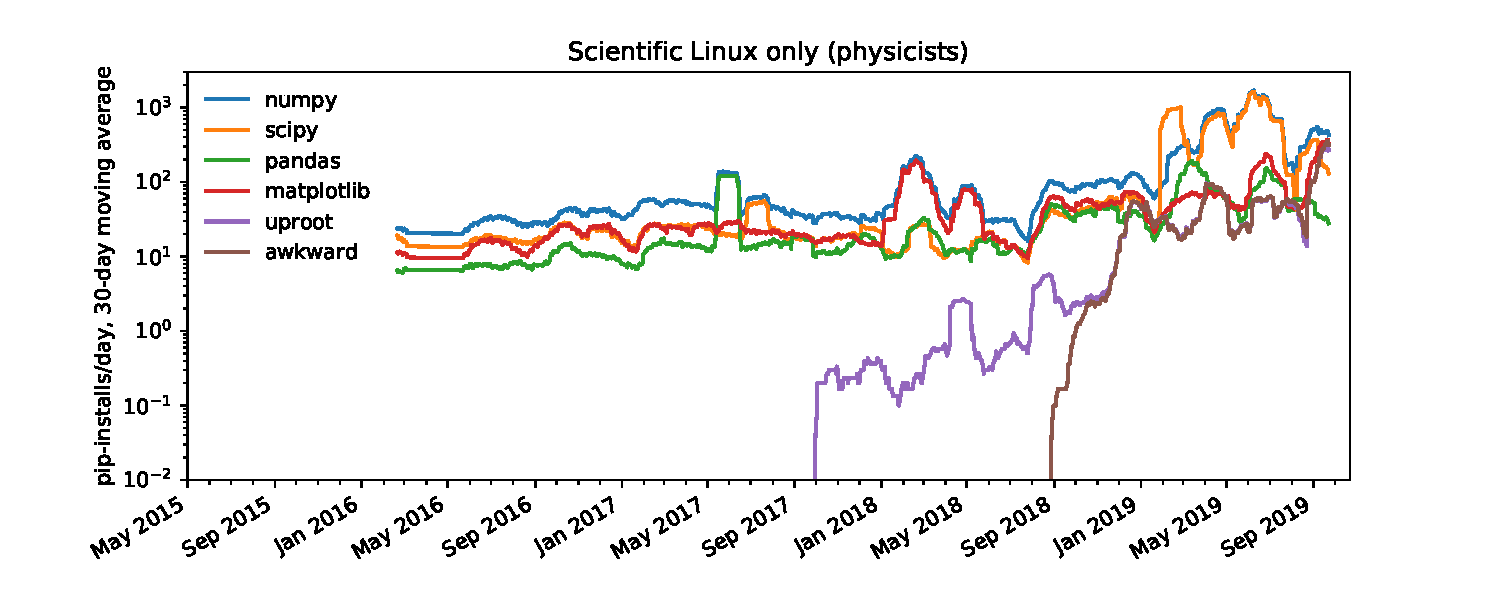
\includegraphics[width=\linewidth]{pip-scilinux-uproot.pdf}}\only<2>{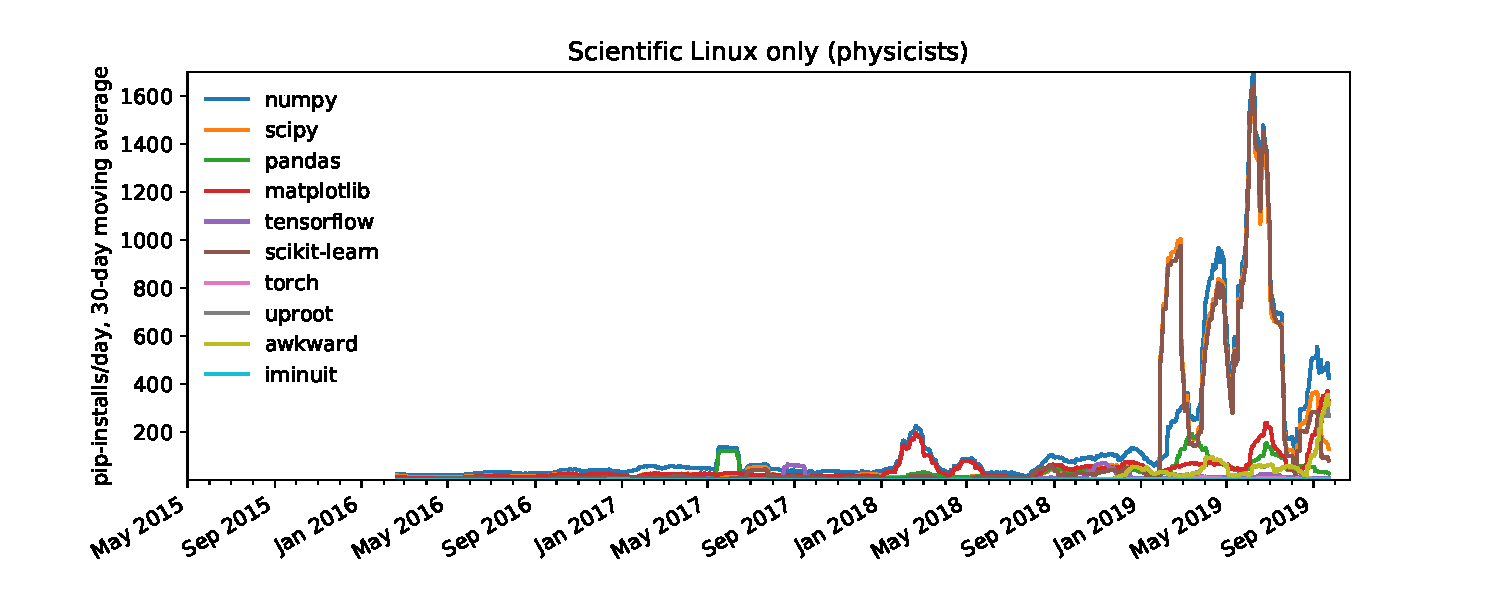
\includegraphics[width=\linewidth]{pip-scilinux-linear.pdf}}\only<3>{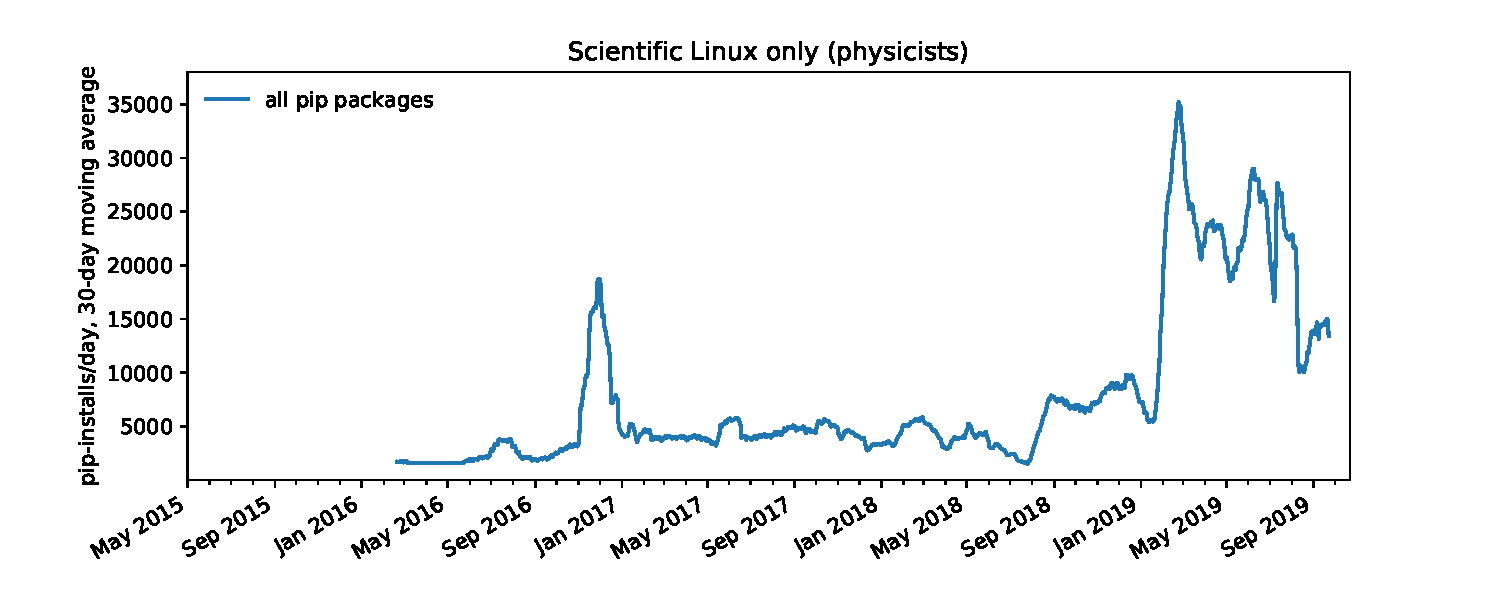
\includegraphics[width=\linewidth]{pip-scilinux-everything.pdf}}\only<4>{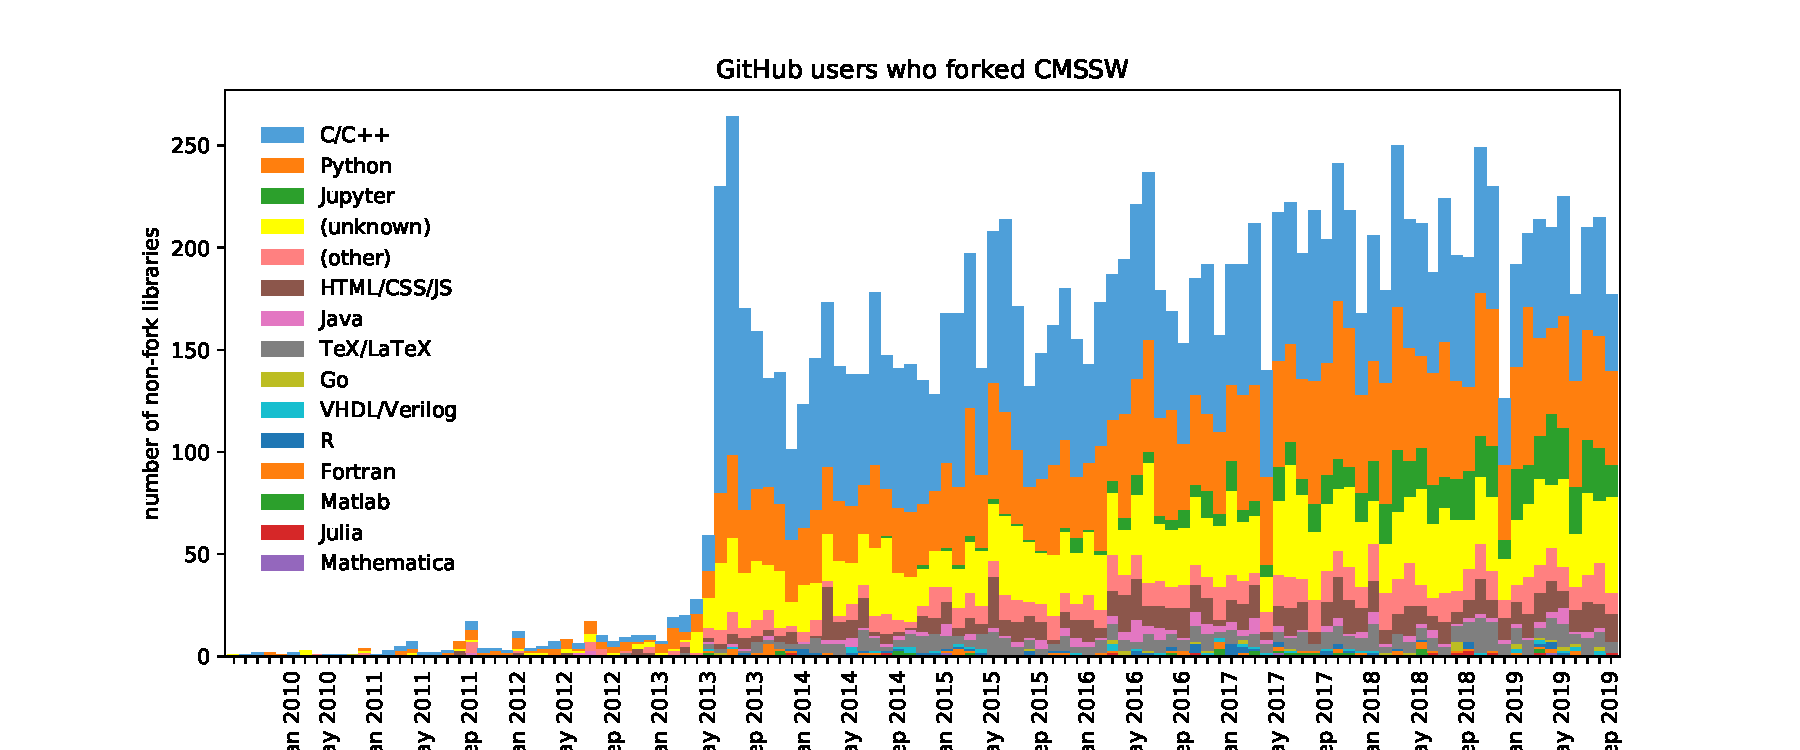
\includegraphics[width=\linewidth]{github-linear.pdf}}\only<5>{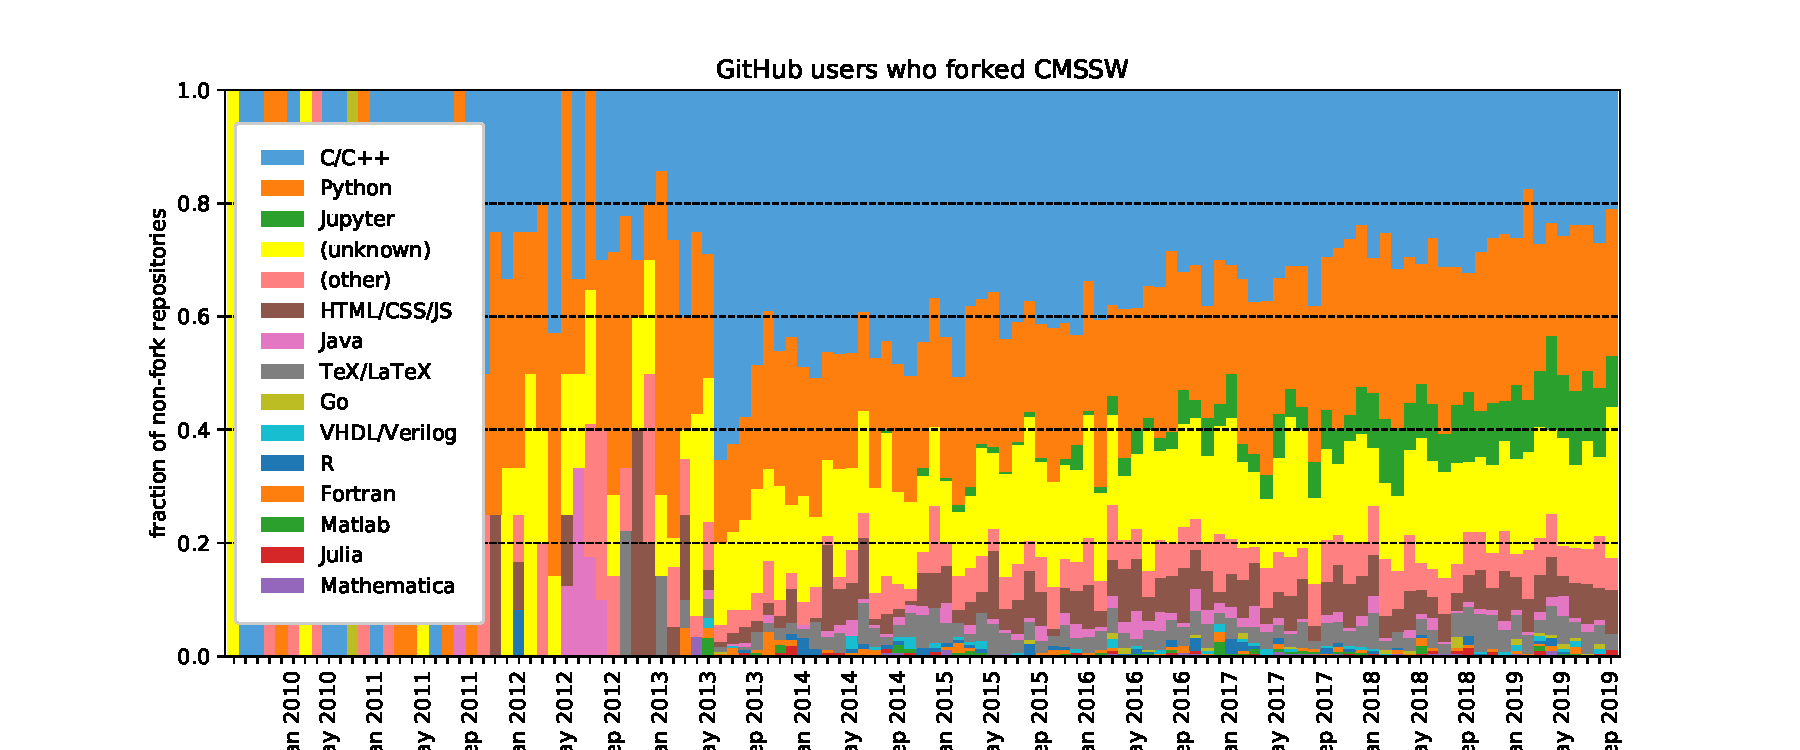
\includegraphics[width=\linewidth]{github-fraction.pdf}}\only<6>{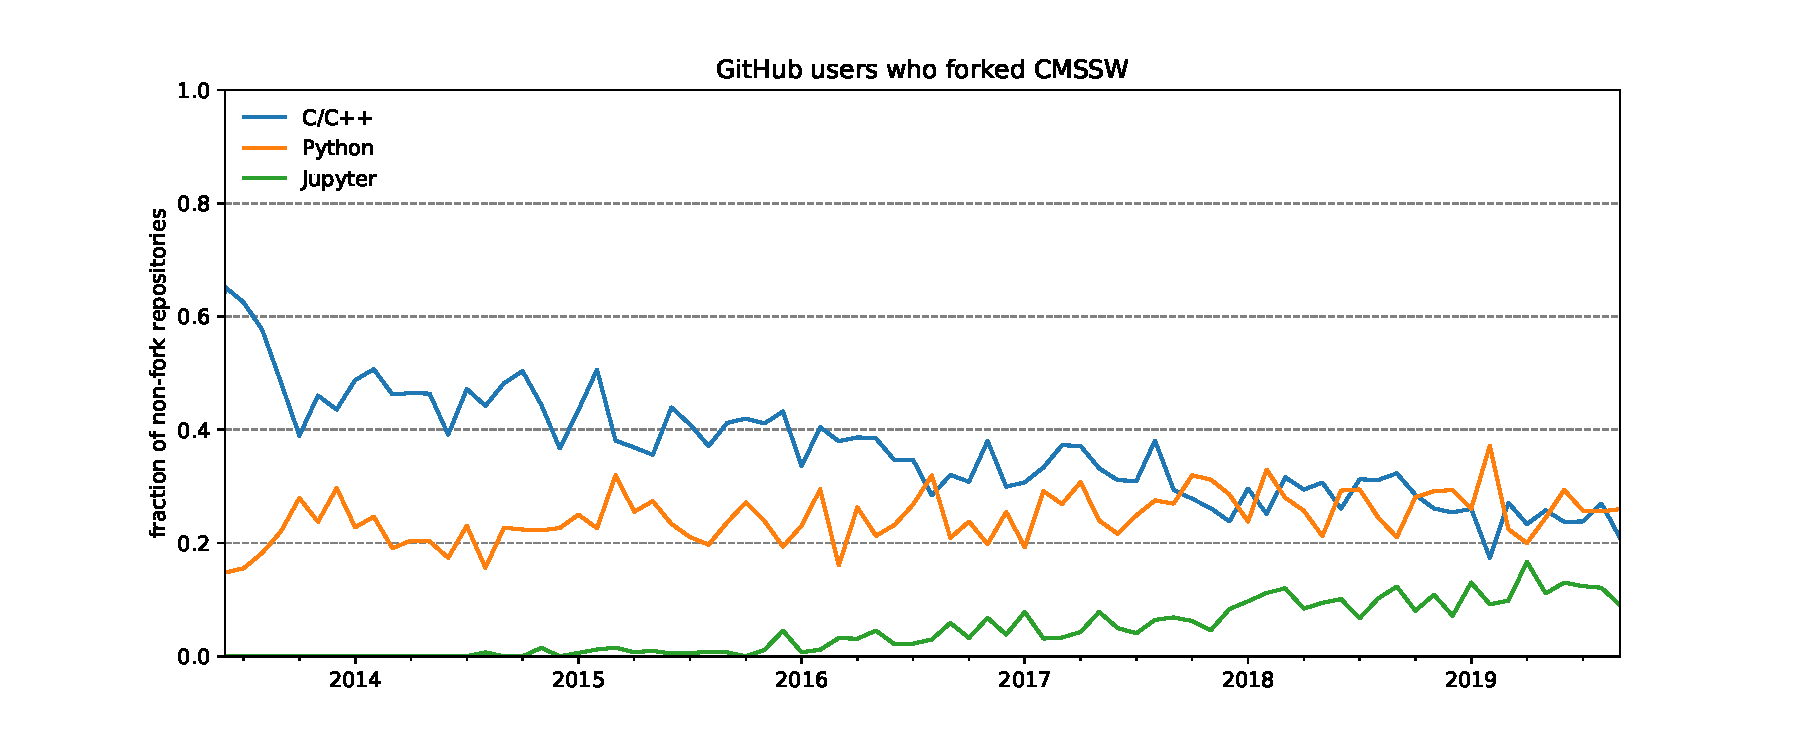
\includegraphics[width=\linewidth]{github-simplefraction.pdf}}\only<7>{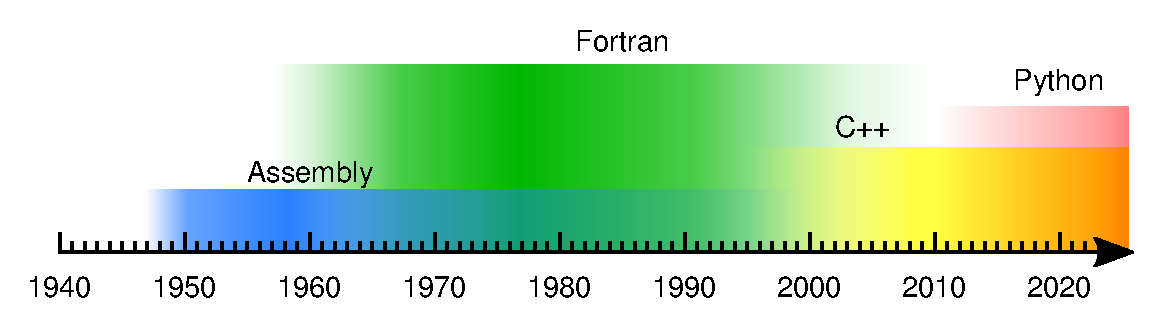
\includegraphics[width=0.95\linewidth]{programming-languages.pdf}}

\begin{onlyenv}<7>
\vspace{-0.75 cm}
\begin{center}
\mbox{\textcolor{darkgray}{predominant programming languages in HEP}\hspace{0.5 cm}}
\end{center}
\end{onlyenv}
\end{columns}
\end{frame}

\begin{frame}{}
\huge
\vspace{1 cm}
\begin{center}
\textcolor{darkblue}{BACKUP}
\end{center}
\end{frame}

\begin{frame}{(Beyond HEP, uproot is 4 orders of magnitude below Pandas)}
\vspace{0.5 cm}
\begin{columns}
\column{1.2\linewidth}
\only<1>{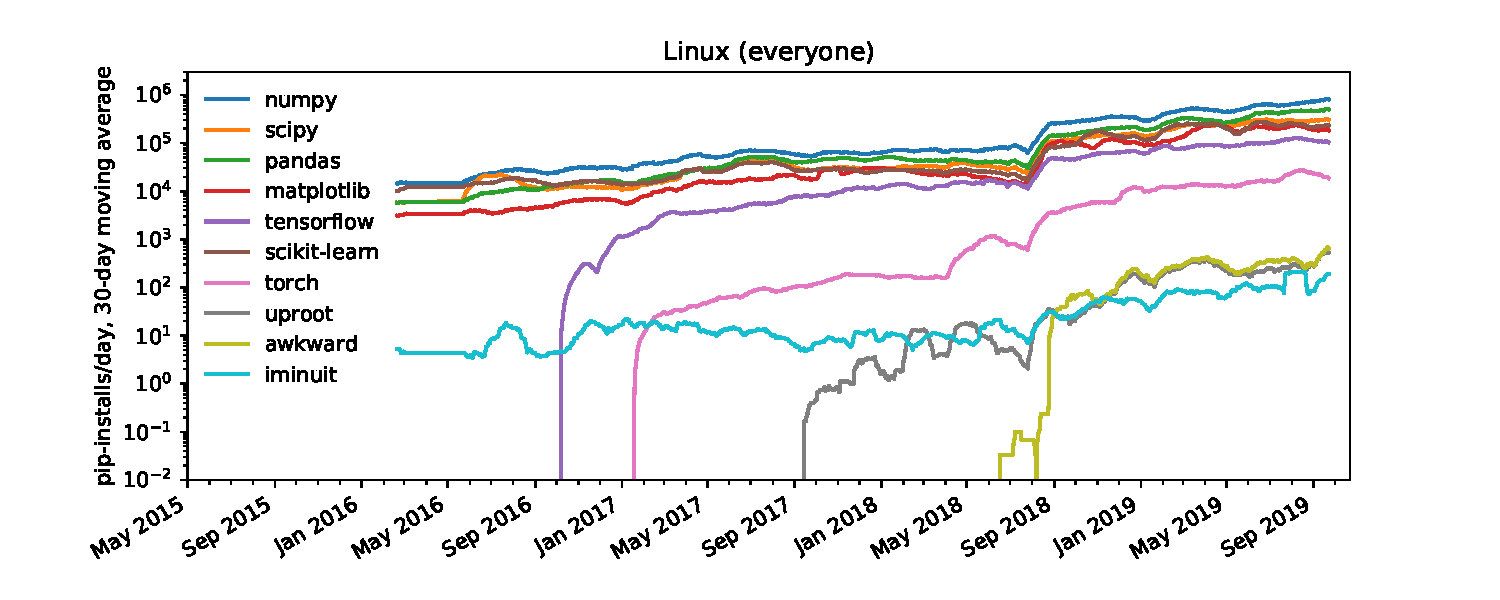
\includegraphics[width=\linewidth]{pip-linux.pdf}}\only<2>{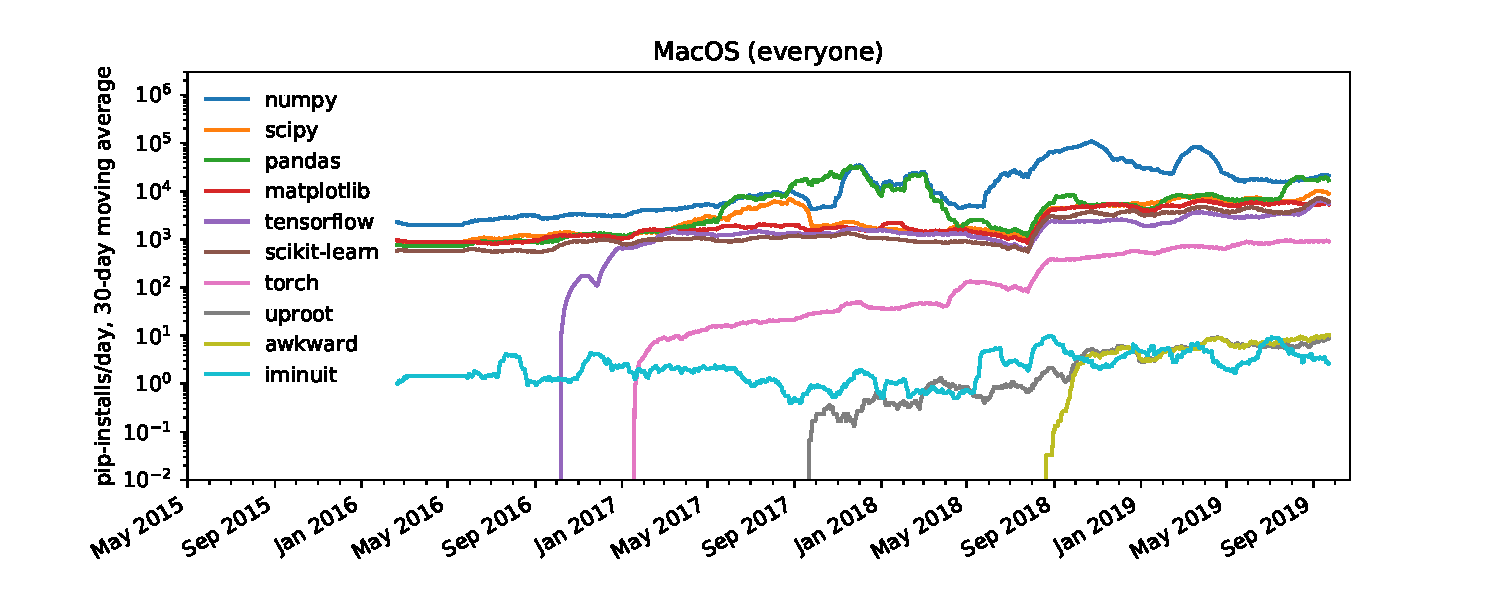
\includegraphics[width=\linewidth]{pip-macos.pdf}}\only<3>{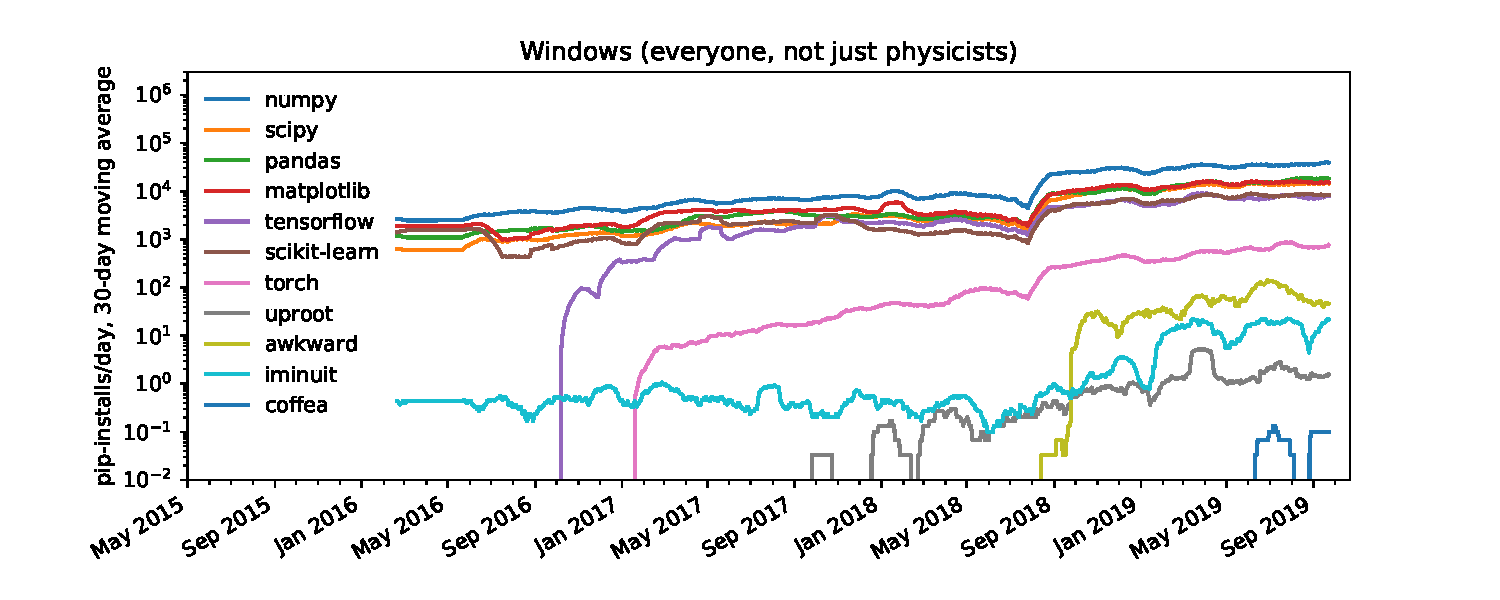
\includegraphics[width=\linewidth]{pip-windows.pdf}}
\end{columns}
\end{frame}

\begin{frame}[fragile]{Analysis of pip download data \only<1-3>{(Google BigQuery)}\only<4>{(GitHub API)}}
\vspace{0.5 cm}
\scriptsize

\textcolor{blue}{\url{https://github.com/jpivarski/2019-10-17-pyhep-awkward/blob/master/analysis.ipynb}}

\vspace{0.25 cm}
\begin{onlyenv}<1>
\begin{minted}{sql}
SELECT
  DATE(timestamp) AS date,
  CASE WHEN country_code = "CH" THEN "CH" WHEN country_code = "US" THEN "US"
       ELSE "other" END AS country,
  file.project AS project,
  REGEXP_REPLACE(file.version, "\\.[0123456789]{1,}$", "") AS version,
  COUNT(*) AS count
FROM `the-psf.pypi.downloads*`
WHERE
  _TABLE_SUFFIX BETWEEN '20160101' AND '20190922'
  AND (file.project = "uproot" OR         file.project = "awkward" OR
       file.project = "iminuit" OR        file.project = "matplotlib" OR
       file.project = "pandas" OR         file.project = "numpy" OR
       file.project = "tensorflow" OR     file.project = "torch" OR
       file.project = "Keras" OR          file.project = "scikit-learn" OR
       file.project = "scipy")
  AND details.distro.name LIKE "%Scientific%" AND details.installer.name = "pip"
GROUP BY project, version, date, country
ORDER BY project, version, date, country
\end{minted}
\vspace{10 cm}
\end{onlyenv}\begin{onlyenv}<2>
\begin{minted}{sql}
SELECT
  DATE(timestamp) AS date,
  details.system.name AS os,
  file.project AS project,
  REGEXP_REPLACE(file.version, "\\.[0123456789]{1,}$", "") AS version,
  COUNT(*) AS count
FROM `the-psf.pypi.downloads*`
WHERE
  _TABLE_SUFFIX BETWEEN '20160101' AND '20190922'
  AND (file.project = "uproot" OR         file.project = "awkward" OR
       file.project = "iminuit" OR        file.project = "matplotlib" OR
       file.project = "pandas" OR         file.project = "numpy" OR
       file.project = "tensorflow" OR     file.project = "torch" OR
       file.project = "Keras" OR          file.project = "scikit-learn" OR
       file.project = "scipy")
  AND details.installer.name = "pip"
GROUP BY project, version, date, os
ORDER BY project, version, date, os
\end{minted}
\vspace{10 cm}
\end{onlyenv}\begin{onlyenv}<3>
\begin{minted}{sql}
SELECT
  DATE(timestamp) AS date,
  CASE WHEN country_code = "CH" THEN "CH" WHEN country_code = "US" THEN "US"
       ELSE "other" END AS country,
  COUNT(*) AS count
FROM `the-psf.pypi.downloads*`
WHERE
  _TABLE_SUFFIX BETWEEN '20160101' AND '20190922'
  AND details.distro.name LIKE "%Scientific%" AND details.installer.name = "pip"
GROUP BY date, country
ORDER BY date, country
\end{minted}
\vspace{10 cm}
\end{onlyenv}\begin{onlyenv}<4>
\begin{minted}{bash}
for x in 1 ... 97; do curl "https://api.github.com/repos/cms-sw/cmssw/forks?page=$x"
  -u 'USERNAME:PASSWORD' > github-cmssw/forks-$x.json; echo $x; done

python -c 'import json, glob; print("\n".join([fork["owner"]["login"] for filename in
  glob.glob("github-cmssw/forks-*.json") for fork in json.load(open(filename))]))'
  > github-cmssw/users.txt

for x in `cat github-cmssw/users.txt`; do curl "https://api.github.com/users/$x/repos
  ?per_page=100" -u 'USERNAME:PASSWORD' > github-cmssw/user-$x.json; echo $x; done

python -c 'import json, glob; print("repo,owner,isfork,created,language"); print("\n"
  .join([",".join(map(str, [repo["name"], repo["owner"]["login"], repo["fork"],
  repo["created_at"], repr(repo["language"])])) for filename in glob.glob("github-cmssw
  /user-*.json") for repo in json.load(open(filename))]))' > github-cmssw.csv

curl "https://api.github.com/repos/scikit-hep/REPOSITORY/issues?state=all&page=PAGENUM
  &per_page=100" >> github-issues-REPOSITORY.json

python -c 'import json; print("number,title,user,state,date_created,date_closed,
  numcomments,ispull"); print("\n".join([",".join([str(x["number"]), json.dumps(
  x["title"]), x["user"]["login"], x["state"], str(x["created_at"]), str(x["closed_at"]),
  str(x["comments"]), str("pull_request" in x)]) for x in json.load(open("github-issues
  -REPOSITORY.json"))]))' > github-issues-REPOSITORY.csv 
\end{minted}
\vspace{10 cm}
\end{onlyenv}
\end{frame}

\begin{frame}{Year of Python, so what do I do? Go back to C++\ldots}
\Large
\vspace{0.5 cm}
\begin{columns}
\column{1.1\linewidth}
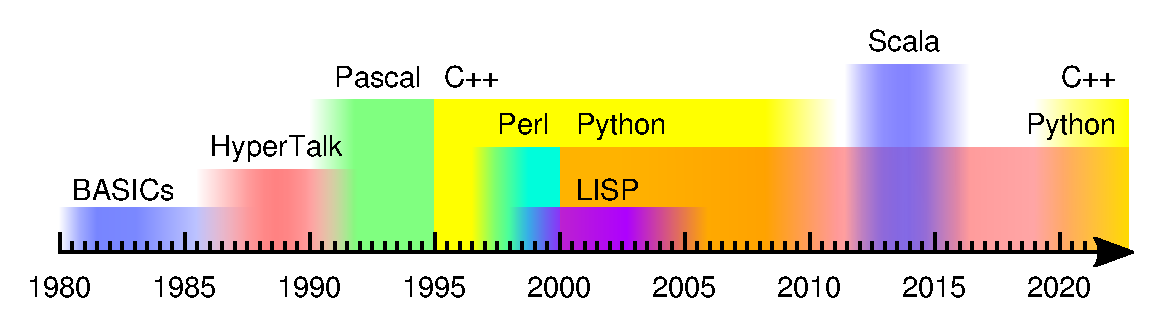
\includegraphics[width=\linewidth]{personal-programming-languages.pdf}

\begin{center}
\vspace{-0.75 cm}
\textcolor{darkgray}{predominant programming languages in my own life}
\end{center}
\end{columns}
\end{frame}

\end{document}
